\documentclass[a4paper]{scrartcl}
\usepackage[utf8]{inputenc}
\usepackage[english]{babel}
\usepackage{graphicx}
\usepackage{lastpage}
\usepackage{pgf}
\usepackage{wrapfig}
\usepackage{fancyvrb}
\usepackage{fancyhdr}
\usepackage{hyperref}
\pagestyle{fancy}

\catcode`\_=\active
\protected\def_#1_{\textit{#1}}

% Create header and footer
\headheight 27pt
\pagestyle{fancyplain}
\lhead{\footnotesize{Network Programming, ID1212}}
\chead{\footnotesize{Android}}
\rhead{}
\lfoot{}
\cfoot{\thepage}
\rfoot{}

% Create title page
\title{Assignment 5 - Distributed Android App}
\subtitle{Network Programming, ID1212}
\author{Bernardo Gonzalez Riede, begr@kth.se}
\date{\today}

\begin{document}

\maketitle

%Introduction
\section{Introduction}
Goals:
\begin{itemize}
	\item Design, develop and deploy an Android app using the Android SDK
	\item Usage of the Android SDK and IDE tools
\end{itemize}


%Literature
\section{Literature Study}
As in previous assignments, the main source were the video lectures on the topic and the example code.

%Literature
\section{Method}
The server side code has been reused from Assignment 1 which uses the MVC approach, having a startup, net (view), controller and model layer.
The client side, an android app, has been developed with Android studio using the Android SDK 26.


\section{Result}

Link to public Github repository with code:
\href{https://github.com/MemBernd/ID1212-Android}{https://github.com/MemBernd/ID1212-Android}

\subsection{Layering}
The app is dived in _main_ and _net_ (work) layer.
The network layer includes the AsyncTasks which handle the connection initialization, sending and receiving.
4 classes are inside the main layer; two activities, a global constants holding class and an _Application_ extending class.


%subsection covering implementation
\subsection{Client \& Server}

\subsubsection{Server}
Being a slightly modified version of the first assignment, the server is a Java implementation of a hangman game.
It creates a new handler for every client connected, identified by the assigned port number, and is therefore multithreaded.
The previously mentioned modification is an inclusion of a header in the server reply to indicate the receiving client if it's a message indicating a (new) state of the game or if its information regarding a prohibited move, e.g. an attempt to solve it with an incorrect amount of characters.

\subsubsection{Client}
On the client side, the android app, the implementation involves mostly GUI operations and network communication.

The _GlobalState_ class extends the _Application_ class, allowing other classes in the process to access this class as a context.
It stores a reference to the _Socket_, _PrintWriter_ and _BufferedReader_. 
An application context is an easy implementation of a temporary form of storage to circumvent the need of passing arguments in the creation of an _Intent_ and dealing with non-serializable objects like sockets.


When trying to connect to the server (MainActivity l. 19) net.EstablishConnection uses the input from the user to try to connect to the server (l. 39 - 44).
After the attempt it calls _onPostExecute_ (l. 55) which either creates an intent to switch to the game activity or displays a toast with a failure indication, based on the previous connection attempt.

Net.Sender takes a String as input an sends it using the PrintWriter from the application context (l. 26).

Net.Listener is called after every sending to process the expected reply from the server.
While _doInBackground_  (l. 31 - 43) only receives the message, _onPostExecute_ (l. 46 - 65) has the necessary logic the act based on the reply from the server.
It shows error or informative messages in the form of toasts or updates the gamestate textview with the information received.

\textbf{Note:}The original idea was to have only one listener start when the game activity is created and let it update whenever something had been received by the server. Trying to do so resulted in the sending task to be executed after the listener finished because of not having received something and therefore timing out. It could be because the emulator uses only a max of 2 threads; one gets used by the UI thread and the other by the AsyncTasks which may get executed sequentially in this case.



%subsection covering gui
\subsection{GUI}

Figure \ref{fig:a1} shows the main activity when launched. 
The user is only taken to the gamestate server if he's able to successfully connect to the server.

\begin{figure}[h!]
  \begin{center}
    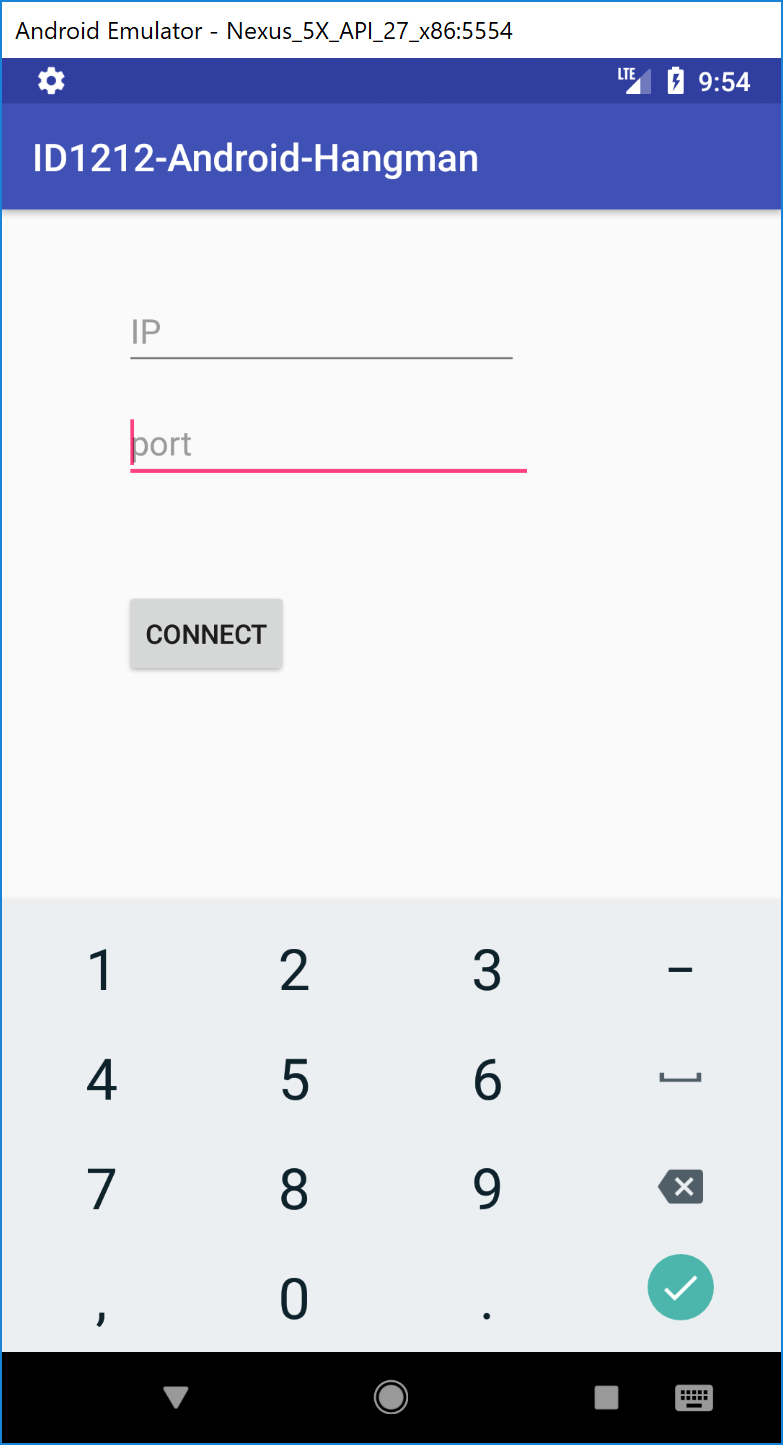
\includegraphics[scale=0.5]{Activity1.png}
    \caption{Initial interface}
    \label{fig:a1}
  \end{center}
\end{figure}


Figure \ref{fig:a2} is an example of a game after a game has been lost already.
In a second iteration it would be easily possible to extract the game score and attempts left counter and create a textview or similar to hold said information separately. Additionally, a afore mentioned toast can be seen at the bottom.

\begin{figure}[h!]
  \begin{center}
    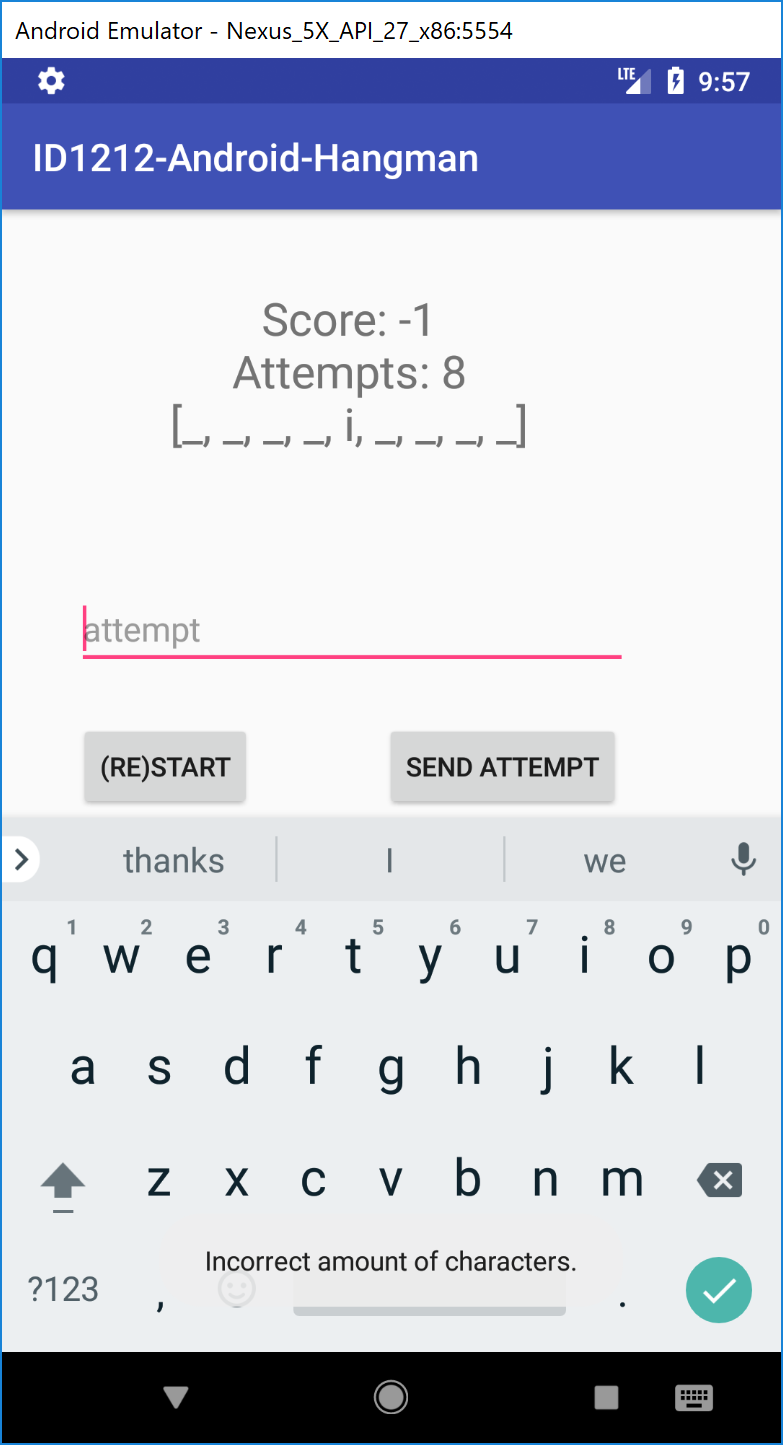
\includegraphics[scale=0.5]{Activity2.png}
    \caption{Game interface}
    \label{fig:a2}
  \end{center}
\end{figure}

%subsection discussion
\section{Discussion}
Some unexpected behaviours were encountered sometimes, e.g. network operations in the UI thread, which are due to the nature of the android framework. 
Still, it wasn't obvious at first and delayed some of the work.

%subsection comments
\section{Comments About the Course}

It took around 7 hours (netto) for the project. 
\begin{itemize}
        \item 4 hours 20 min for coding.
        \item 1 hour 15 min for the report.
        \item 1 hour 23 min watching videos, taking notes and thinking about how to tackle the problem.
\end{itemize}




\end{document}
